%\textcolor{red}{Kurze Hinweise auf die Änderungen, die ich gemacht habe.
%\begin{itemize}
%    \item anpassung der neuen "views" in section "interactive functionalities" (rot-coloriert)
%    \item generelle anpassung der figures durch
%	\begin{itemize}
%	    \item einfügen der URLs: weiß nicht, ob das so gut aussieht mit dem TExt, also ggf
%		einfach ändern, oder nur reduzieren auf die URL in Klammern (?)
%	    \item verlinken der images mit dem hyperlink, damit ein Klicken sofort zur Website
%		führt. Ob das was bringt, hängt davon ab, wie LREC die PDFs einbindet. Wenn es nicht
%		klappt, ist das schade, aber verkraftbar
%	\end{itemize}
%    \item ich habe auch die grafiken anpassen müssen, weil die PDF-Struktur "gecroppt" ist (oder wie
%	man das nennt), jedoch nach wie vor die alte Seitengröße enthält. Um das zu umgehen, habe
%	ich sie mittels pstricks noch mal explizit eingebunden (siehe wheel-image.pdf). Visuell
%	macht das keinen Unterschied, aber der HREF ist jetzt auf dem ganzen Bild aktiv, und nicht
%	nur auf einzelnen Teilen
%    \item ich habe auch figure 5 auf die seite gedreht, weil sie mir zu groß war und ich auch den
%	Unterschied schlecht erfassen konnte. Ich finde, dass er in der jetzigen form praegnanter
%	ist und man besser den unterschied erkennt.
%\end{itemize}
%Lösch diesen Text und die anderen Rot-Stellen einfach, wenn du dir dies hier angeschaut hast. 
%Grüße, Mattis}
The CLICS database is available online at \url{http://clics.lingpy.org} and offers its users a search interface to all concepts and crosslinguistic colexifications between concepts. The wealth of information in the database and the various possibilities of exploring the colexifications in the network call for an additional component that makes potentially interesting observations more easily accessible to the researcher. The idea was to equip the database with a visualization component that provides various interactive functionalities and enables users to navigate through the networks of colexifications while at the same time providing more detailed information on the actual language data. 
%A prototype of the visualization is online accessible.\footnote{\url{http://tinyurl.com/clicsvis}}
\nocite{Wold2009,Key2007}
\subsection{Web-based visualization}
% why web-based? main advantages

We opted for a web-based implementation of the CLICS visualization in JavaScript using the D3 library \cite{D3}. The main benefits of a web-based visualization are its platform independence and the fact that users can access it from any device with a browser supporting JavaScript. There is no need for the installation of additional software or for maintenance of the system on the part of the user \cite{Murray}. In addition, links to the descriptions of the external resources can easily be included to allow users to explore the CLICS data in more detail on demand. 

\subsection{Data preparation}
In its current form, the data in CLICS yields a \emph{small world network} in which all nodes are
densely connected. Browsing such a dense network is very confusing and provides few insights for
the user (see Figure \ref{fig:clics_full}). In order to break down the complexity inherent in CLICS,
we employed two different strategies to present the data from two different perspectives. 
According to our first strategy, we decided to split the data
into \emph{communities} first. 
Starting from 1,280 concepts in CLICS which
were connected to at least one other concept, we applied the \emph{Infomap} algorithm by
\newcite{Rosvall2008} to cluster all concepts into communities.
The \emph{Infomap} algorithm requires that weights are defined for the edges of the network.
Here we used the number of attested language families per colexification as edge weights. Following
a suggestion by \newcite{Dellert2014} we
further normalized the number of attested language families with the help of Formula \ref{Formula}:
\begin{equation} \label{Formula}
    W = \frac{C^2}{O_A+O_B - C},
\end{equation}
where $C$ is the number of attested language families for the colexification of concept $A$ and
concept $B$, $O_A$ is the number of language families in which concept $A$ occurs, and $O_B$ is the
number of language families in which concept $B$ occurs. 
The \emph{Infomap} algorithm was chosen because of
its remarkable performance on the community detection task, both in terms of computation time and
quality of results \cite{Lancichinetti2009}.
With the help of this analysis, it was possible to subdivide the 1,280 concepts into 271 communities. 
Of these communities, 118 are \emph{large}, containing more than
five nodes. The large communities cover 65\% (828) of all nodes in the original network (1,280). In
order to enable the user to quickly identify communities of specific interest, we labeled all
communities by taking the concept with the highest degree as representative. 
The communities do not differ much in size, ranging from 2 (`men's house') to 16 concepts (`{fur}')
with an average of 4.72 concepts per community.
 
The advantage of the community perspective on CLICS is that it provides an independent automatic
clustering of the data. The disadvantage is that this preselection deprives the user of finding
alternative, possibly interesting connections between the concepts. Community detection methods are not
error-proof, and their performance varies depending on the algorithms being used and the data being analyzed.
Even more importantly, most community detection methods are based on restricted decisions when
clustering the nodes of a given network into groups. Every node is assigned to one community only.
No transitions between communities are possible. In order to offer a less biased perspective on the
network, we decided to extract subgraphs for each concept in the data showing its strongest
connections up to a certain depth of resolution. The individual subgraphs were constructed as follows: starting
from a given concept, we first searched for all of its direct neighbors with which it shared at
least 5 colexifications in five different language families. The same procedure was applied to all neighbors
which were added to the subgraph in the first run and repeated two times. If the resulting graph for a given concept was
too small, a relaxed threshold of 4 colexifications in four different language families was used.  
In the resulting subgraphs, the longest possible path length between the selected concept and all other
concepts is 3. Having excluded 280 subgraphs in which no stronger links between the selected concept and any
other concept could be found, this procedure left us with 1,000 individual subgraphs of individual
size and structure, ranging from 56 nodes (selected concept `take') to 2 (selected concept `north'). 
When browsing the network representation of the data, the user can select between both perspectives
on the data in CLICS, the community perspective, and the perspective of the strongest connections.

\begin{figure}[b]
    \centering
   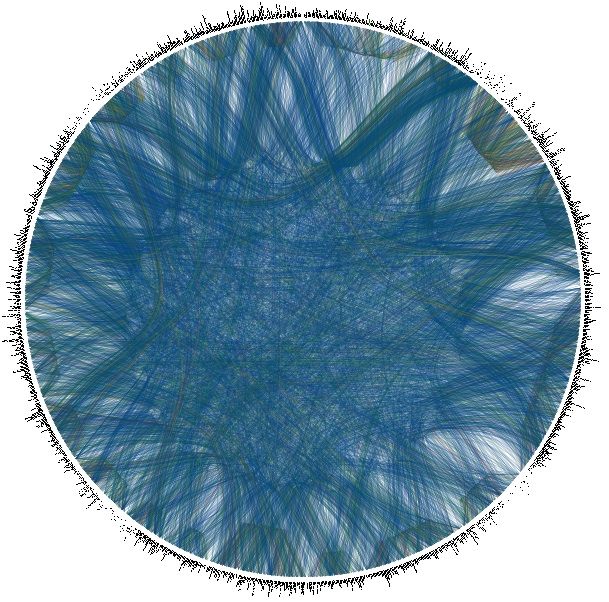
\includegraphics[width=0.48\textwidth]{img/completeNetworkLabels.jpg}
    \caption{Full network of all 1,288 concepts in CLICS (outer circle) together with their connections. The strength of the connections is marked in different colors, with very strong links represented in red}
    \label{fig:clics_full}
\end{figure}


\subsection{Interactive functionalities}


% Force-directed graph; move nodes to desired position

The visualization features various interactive functionalities that are designed to enhance the exploration of the CLICS data at the level of communities or strongest connections. The main component is a flexible force-directed graph layout that displays the concepts as nodes and the crosslinguistic colexifications as edges (see Figure \ref{EarthLand}). The strength of the force in the edges of the graph is dependent on the number of language families that can be attested to having lexical associations for the respective concepts that are linked through the edge. As mentioned in the previous section, we decided to provide two different views on the network, one for separate communities obtained from the \emph{Infomap} analysis \cite{Rosvall2008}, and one in which the subgraph containing the strongest links for each concept is displayed.  With the help of the web interface for network browsing (\url{\clics{browse.php}}) the user can look up the respective subgraphs by selecting the concept of interest and specifying the desired `view.'

\begin{figure}[htbp]
    \centering
    \href{\clics{browse.php?gloss=earth,\%20land}}{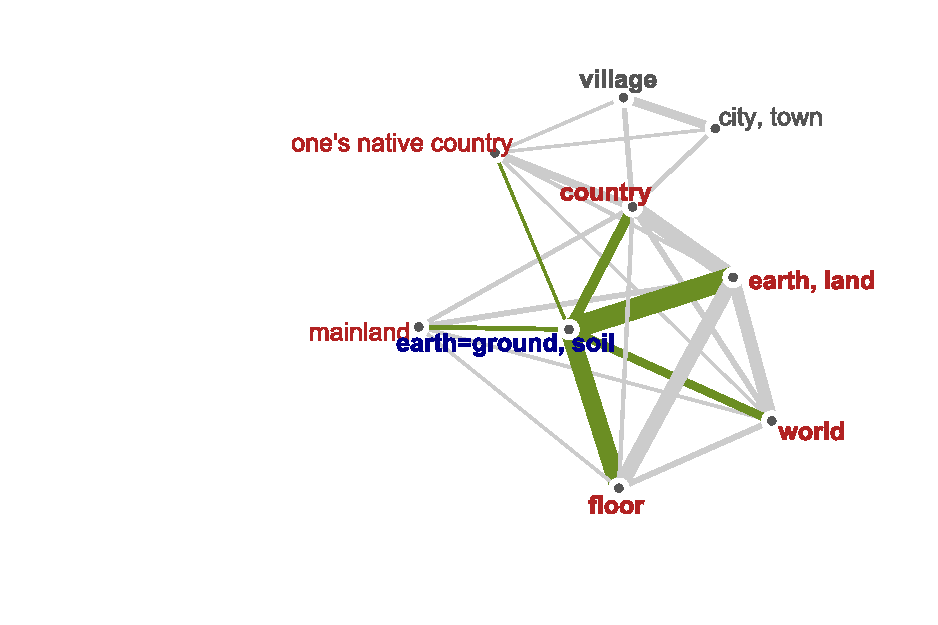
\includegraphics[width=0.48\textwidth,trim=5cm 2cm 1cm 1cm]{img/earthland2.pdf}}
\caption{Force-directed graph with mouse-over functionalities highlighting all connected concepts.
In order to browse the graph on the CLICS website, use the following URL: \url{\clics{browse.php?gloss=earth,\%20land}}.}
\label{EarthLand}
\end{figure}

The force-directed graph layout ensures that all concepts are neatly arranged according to their similarity as defined by the number of crosslinguistic colexifications. As a result, concepts that are highly connected are located close to each other.  To make it easier for users to explore the network that is depicted in the graph, concepts can be dragged to different positions where there is less overlap. The dragging behavior of a concept  is activated when mousing over the respective node in the graph (when the cursor symbol turns into a cross hair). 

\begin{figure*}[htbp]
\begin{center}
    \href{\clics{browse.php?gloss=money&view=part}}{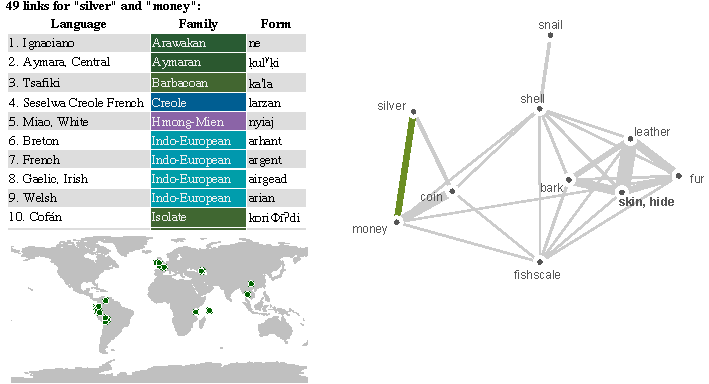
\includegraphics[width=\textwidth]{img/silver-image.pdf}}
\caption{Force-directed graph with mouse-over functionalities showing the strongest links of the
concept `{money}.' The entries have different background colors depending on their location in the
world map (cf. Figure \ref{World map}). In order to browse the graph on the CLICS website, use the
following URL: \url{\clics{browse.php?gloss=money&view=part}}.}
\label{MoneySilver}
\end{center}
\end{figure*}



% mouse-over: coloring edges, show linked languages

As mentioned above, the edges of the graph represent the number of cases of crosslinguistic colexifications for the linked concepts. For a more detailed view on which languages contribute to the strength of the connections, the user can mouse over the links in the graph to see the forms in the individual languages responsible for the associative link (Figure \ref{MoneySilver}). The list includes additional information on the languages such as their ISO 639-3 language code and family. Furthermore, each entry in the list provides a hyperlink to the original source from where the information is taken.  

% Color coding: families and geolocations

Each language in the list is attributed a different background color depending on its language family or location in order to allow for an at-a-glance overview of all languages in the list. The user can choose from a drop-down menu whether to include the genealogical or areal information as the background color. For the genealogical information, all language families are attributed a different color value. Languages belonging to the same language families are therefore given the same background color. Moreover, the list is sorted according to language families. In this way, the user can immediately see how many languages of  a given family contribute to the overall strength for the connection at hand. 

As to the areal information, the world map is provided with a color gradient as shown in Figure \ref{World map}. To this end, each position in the world map is attributed a color value using the L*a*b* color space. The color hue thereby indicates the position on the map in terms of the longitude (specifying the east-west position) whereas the lightness of the color represents the position in terms of the latitude information (specifying the north-south position).\footnote{See \newcite{MayerLanguageExplorer} for a different approach of a linguistically informed color gradient of the world map.}
The mapping from geolocation to color values allows for an easier evaluation of areal patterns in the selected connection. In this regard, users can directly detect whether a certain pattern of colexification is restricted to a certain region of the world or constitutes a more widespread colexification pattern (see the case study in Section \ref{case study} below). In addition, all languages in the list are displayed with their geographical location on a world map (see Figure \ref{MoneySilver}). Hence, areal patterns can be directly compared to the genealogical information in the list (if the first option is chosen).

\begin{figure}[htbp]
\begin{center}
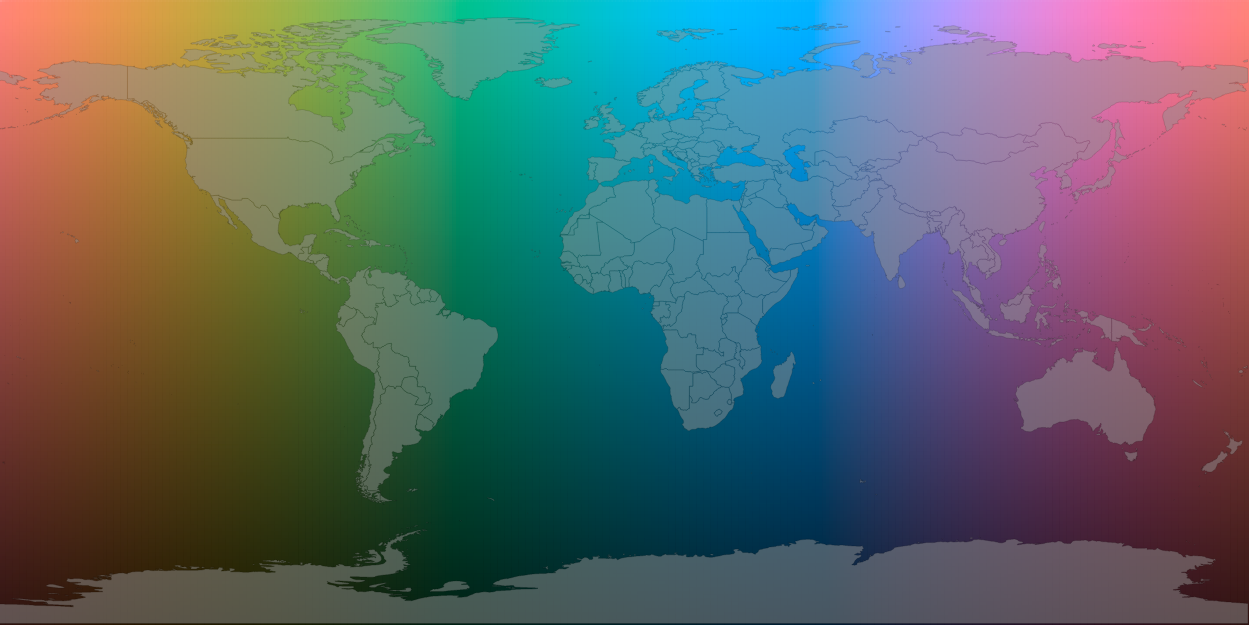
\includegraphics[width=0.48\textwidth]{img/ColorScaleWorld.png}
\caption{World map with color gradient. The color represents the location where a language is spoken (see Figure \ref{MoneySilver} where the background color identifies the location of the language)
%\textcolor{red}{maybe add a small explanation sentence here,probably with a backreference to figure 3, or somehting similar}
}
\label{World map}
\end{center}
\end{figure}


% show only edges with a minimum number of links

In addition to the interactive functionalities described above, the visualization also features a variety of further components that allow for an easier exploration of the database. The graph layout is equipped with panning and zooming functionality that enables the user to navigate through the network graph. Panning is enabled when the cursor changes into a hand symbol when mousing over a link of the graph. The whole graph can then be dragged to a new position. The zooming behavior is activated with the scroll wheel. 
When mousing over a concept (node) in the graph all connected links and concepts are highlighted
in order to provide a better overview of the connectivity of certain concepts (see Figure \ref{EarthLand}). The control panel of the visualization also includes a slider button that allows the user to show only those edges in the graph with a minimum number of crosslinguistic colexifications. 

% zooming and panning



\subsection{Implementation}
% description of D3 and the implementation

The visualization is implemented in JavaScript using the D3 library \cite{D3}.\footnote{\url{http://d3js.org}} The force-directed graph is  generated with the \texttt{force()} function from the \texttt{d3.layout} module. The layout implementation uses position Verlet integration for simple constraints \cite{Dwyer2009}.\footnote{See \url{https://github.com/mbostock/d3/wiki/Force-Layout} for a description of the implementation.} In order to ensure that the concept labels are located close to the concept nodes, a second force layout (with a static weight of $1$) is set up for each concept link to the node. 

The color values for the world map gradient scale are computed from the two-dimensional geographical coordinates that are given as an input. The latitude [-90;90] and longitude [-180;180] values are thereby normalized between [0;1] and serve as the input for the function \texttt{cl2pix}.\footnote{The code was adapted from the GNU C code by David Dalrymple (\url{http://davidad.net/colorviz/}, accessed on January 25, 2014) and translated into JavaScript.}

\begin{verbatim}
function cl2pix(c,l){
   		var TAU = 6.2831853 
   		var L = l*0.61 + 0.09; 
   		var angle = TAU/6.0 - c*TAU;   
   		var r = l*0.311 + 0.125 
   		var a = Math.sin(angle)*r;
   		var b = Math.cos(angle)*r;
   		return [L,a,b];
 };
\end{verbatim}

The actual HTML color code is generated with the function \texttt{d3.lab} from the D3 library, which takes the three values for \texttt{[L,a,b]} as input. The main reason for choosing the L*a*b* color space is a smoother transition between different color hues without any visible boundaries. As can be seen in Figure \ref{lab vs hsv}, the color gradient in the L*a*b* color space exhibits a much smoother perceptual transition between the color hues on the x-axis. 
%\footnote{See \url{http://davidad.net/colorviz/} for the difference between using the L*a*b* and HSV color space in terms of transitions between different color hues.} 
For the coloring of the language families, the background colors are generated with the categorical scale functions of the \texttt{d3.scale} module. 

\begin{figure}[h]
    \centering
   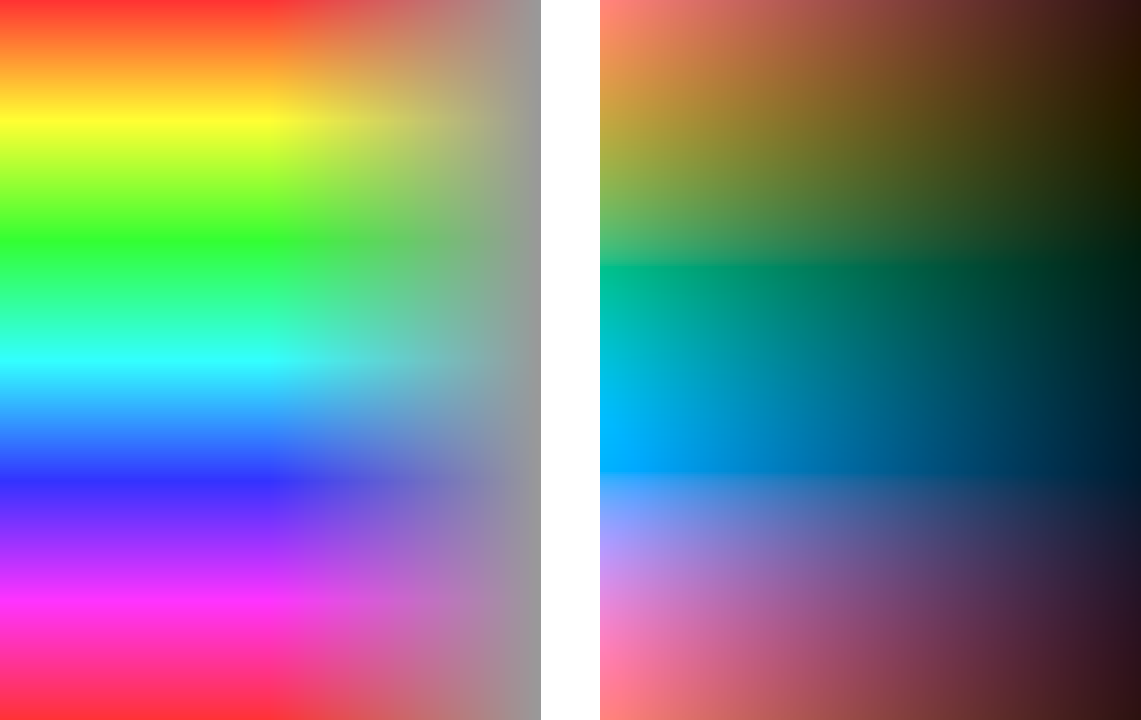
\includegraphics[width=0.48\textwidth]{img/Lab_HSV2.png}
    \caption{Comparison between two-dimensional color gradients in the L*a*b* (right) and HSV (left)
    color space.}
    \label{lab vs hsv}
\end{figure}


The  dragging and panning functionalities of the graph are implemented with the \texttt{drag()} function from the \texttt{d3.behavior} module and the SVG \texttt{transform} and \texttt{translate} attributes. The interactive world map is generated with the \texttt{topojson} package and makes use of the \texttt{d3.geo} projection module.

\subsection{Case studies} \label{case study}

In order to illustrate the usefulness of the visualization for the purposes of exploring the database, consider the graph in Figure \ref{MoneySilver}. Among other things, it contains the connection between the concepts `money' and `silver.' A subset of the languages and words contributing to this connection are shown on the left where the background color represents the location of the languages. For instance, French contributes to the crosslinguistic colexification because both concepts are realized by the same word (viz. \textit{argent}) in that language. When looking at the areal distribution of the languages, a clear pattern emerges at a glance (see Figure \ref{MoneySilverAreas} for the full list of languages showing this colexification pattern). Most of the languages contributing to the colexification are from two major regions: Caucasus (marked in blue) and South America (marked in green). However, as mentioned in Section \ref{caveats}, this distribution might be an artifact of the general bias for languages of the Caucasus and South America in the underlying databases. In any case, the visualization directly points the attention to this pattern. As the  aim of the visualization component is not to replace linguistic research but to guide it, such patterns have to be looked at in more detail by checking the actual data. 

\begin{figure}[htbp]
%\begin{center}
%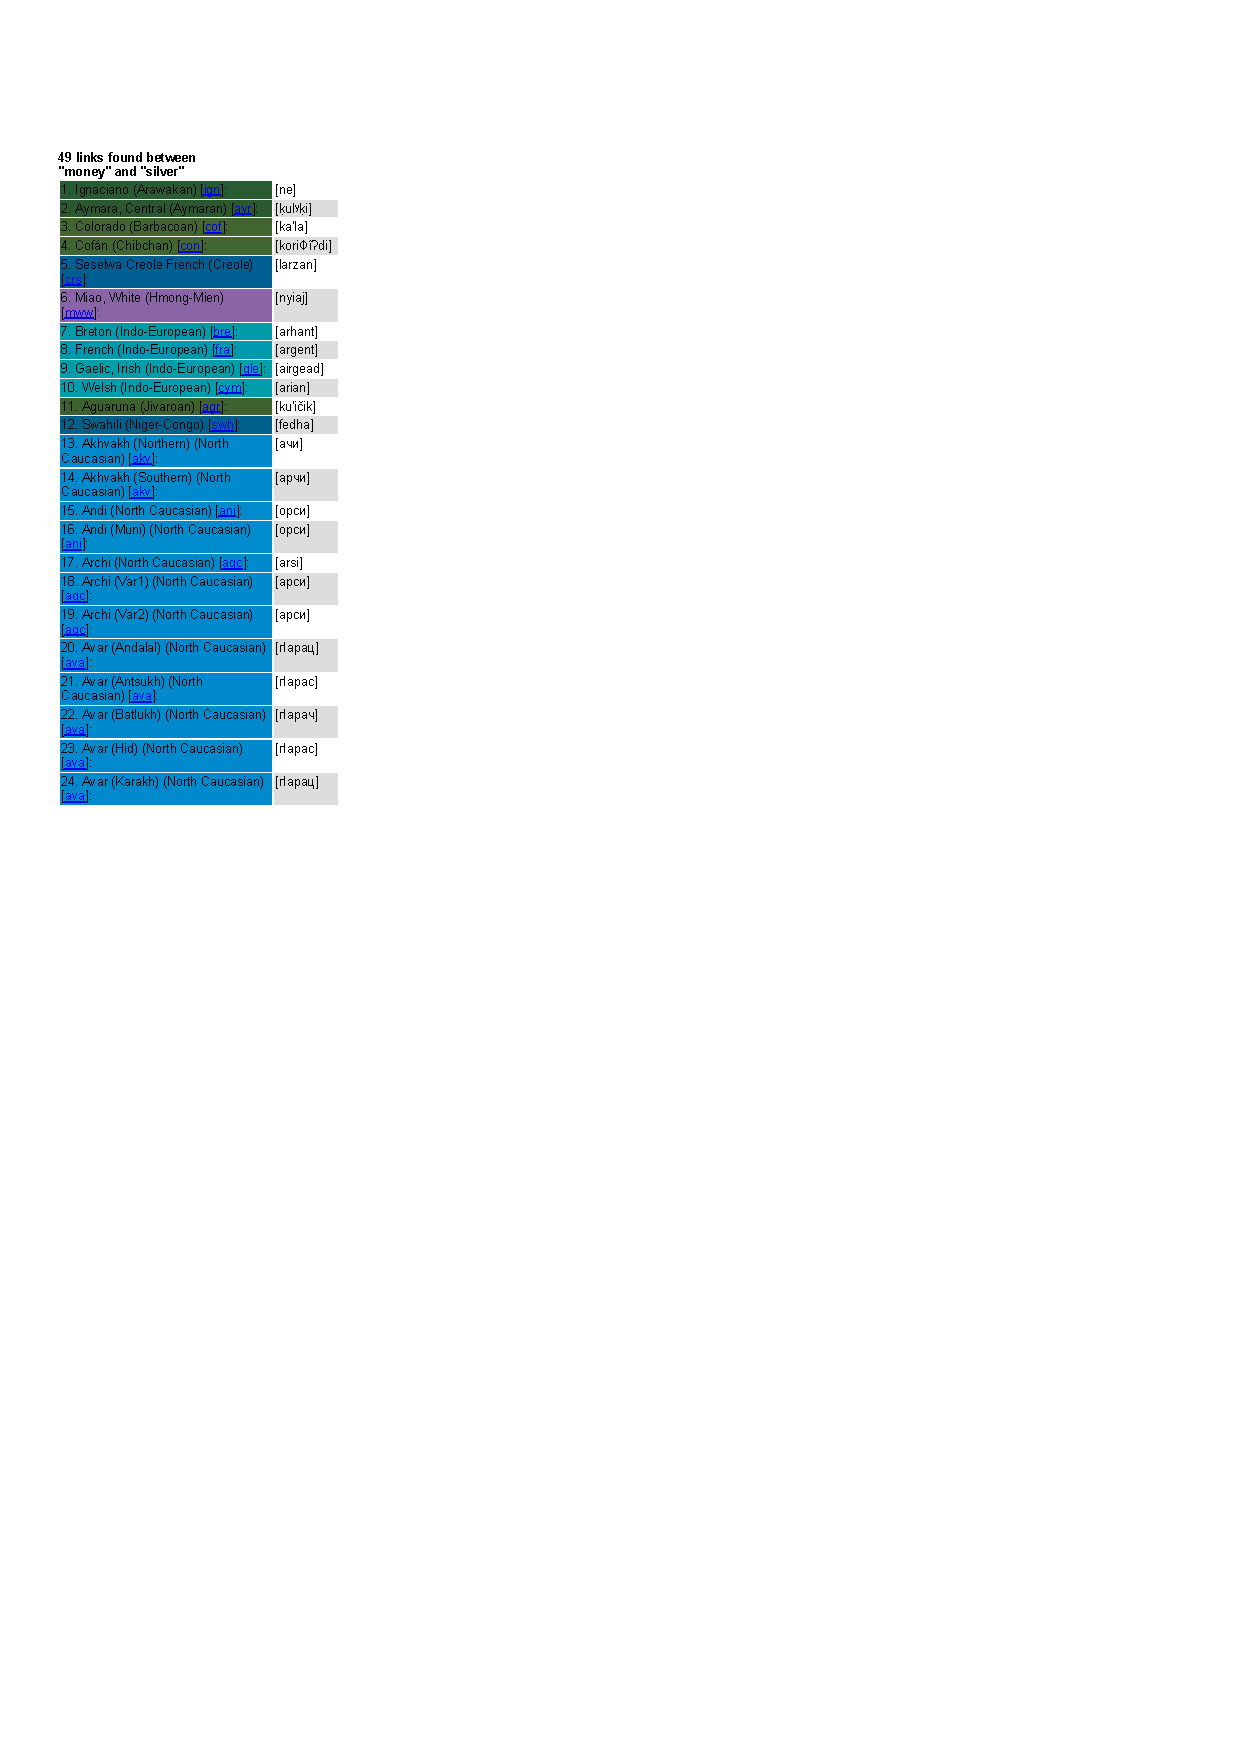
\includegraphics[width=0.238\textwidth]{img/moneysilverAreas1.pdf}
%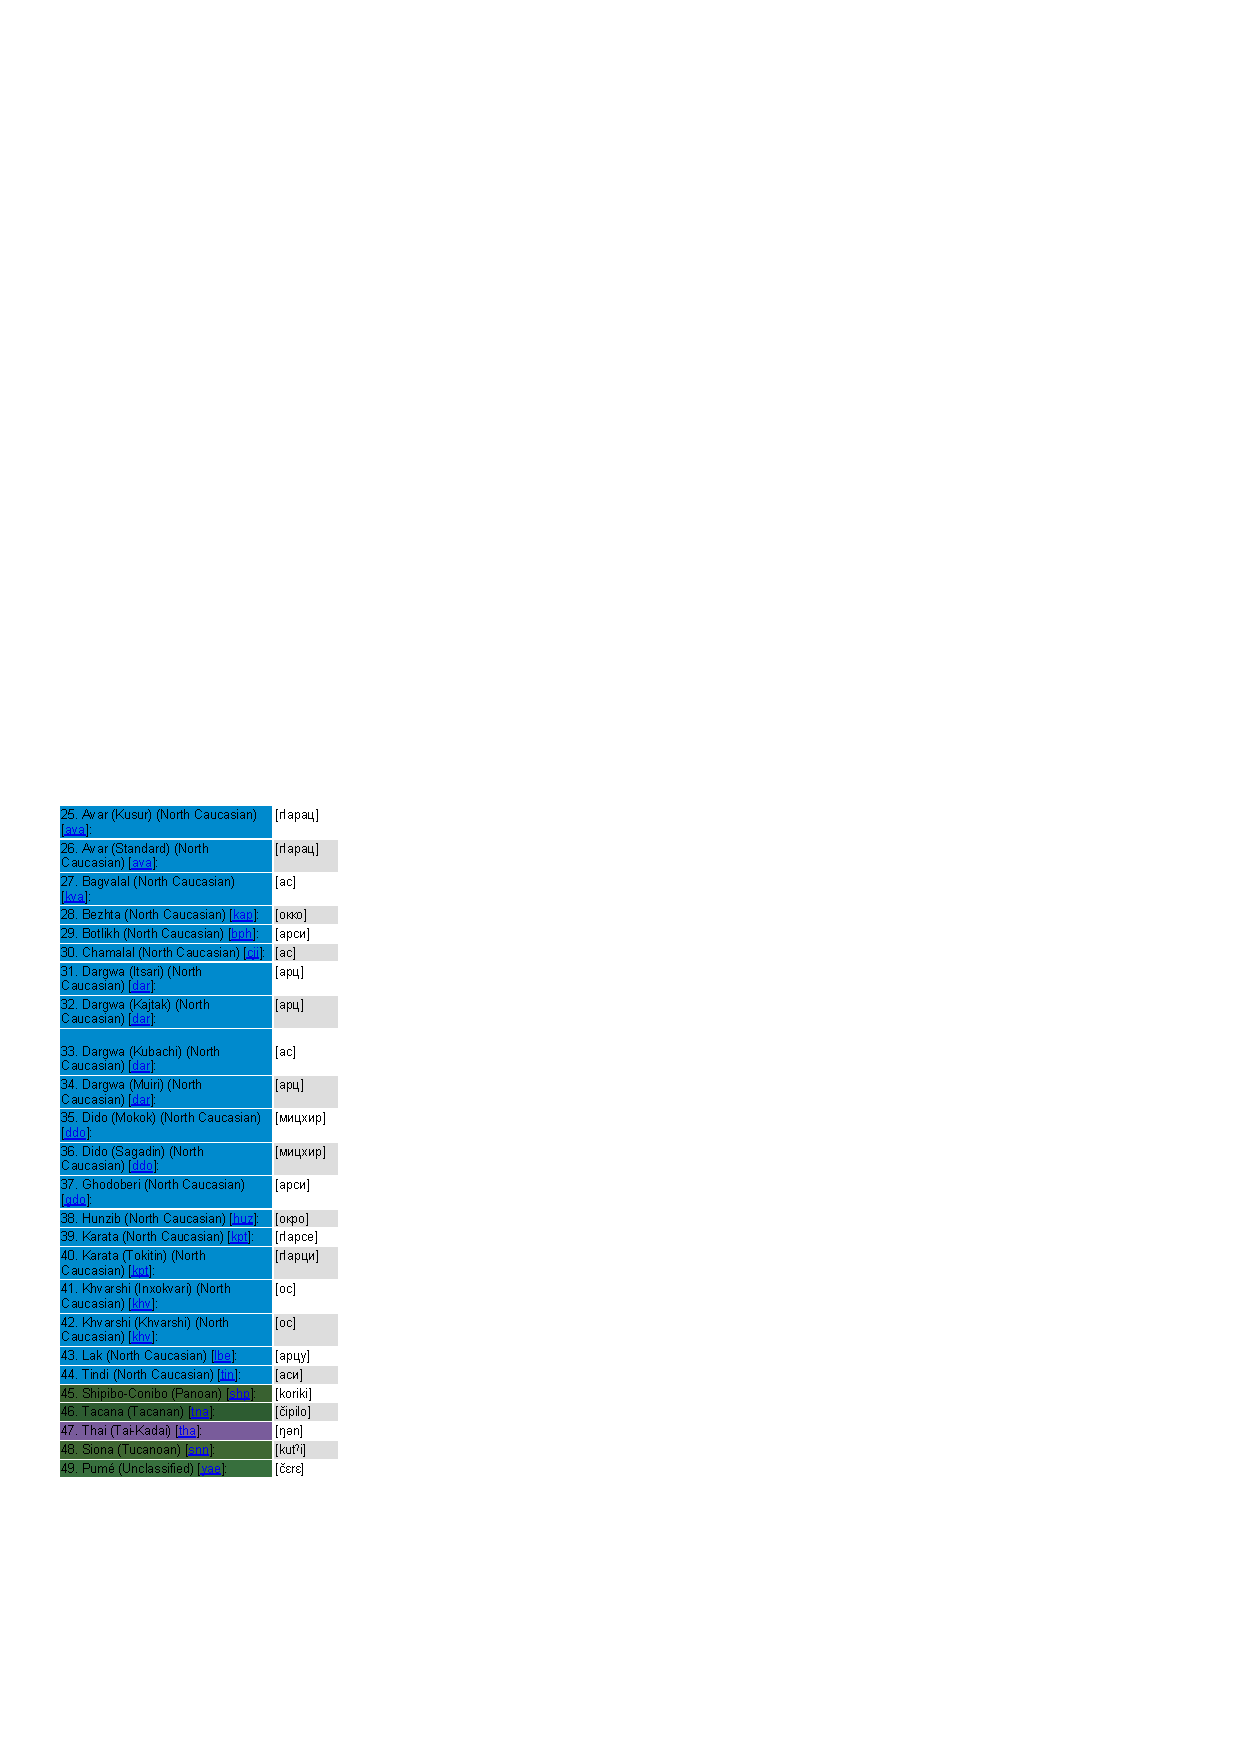
\includegraphics[width=0.238\textwidth]{img/moneysilverAreas2.pdf}
\hspace{-0.4cm}
\begin{tabular}[t]{ll}
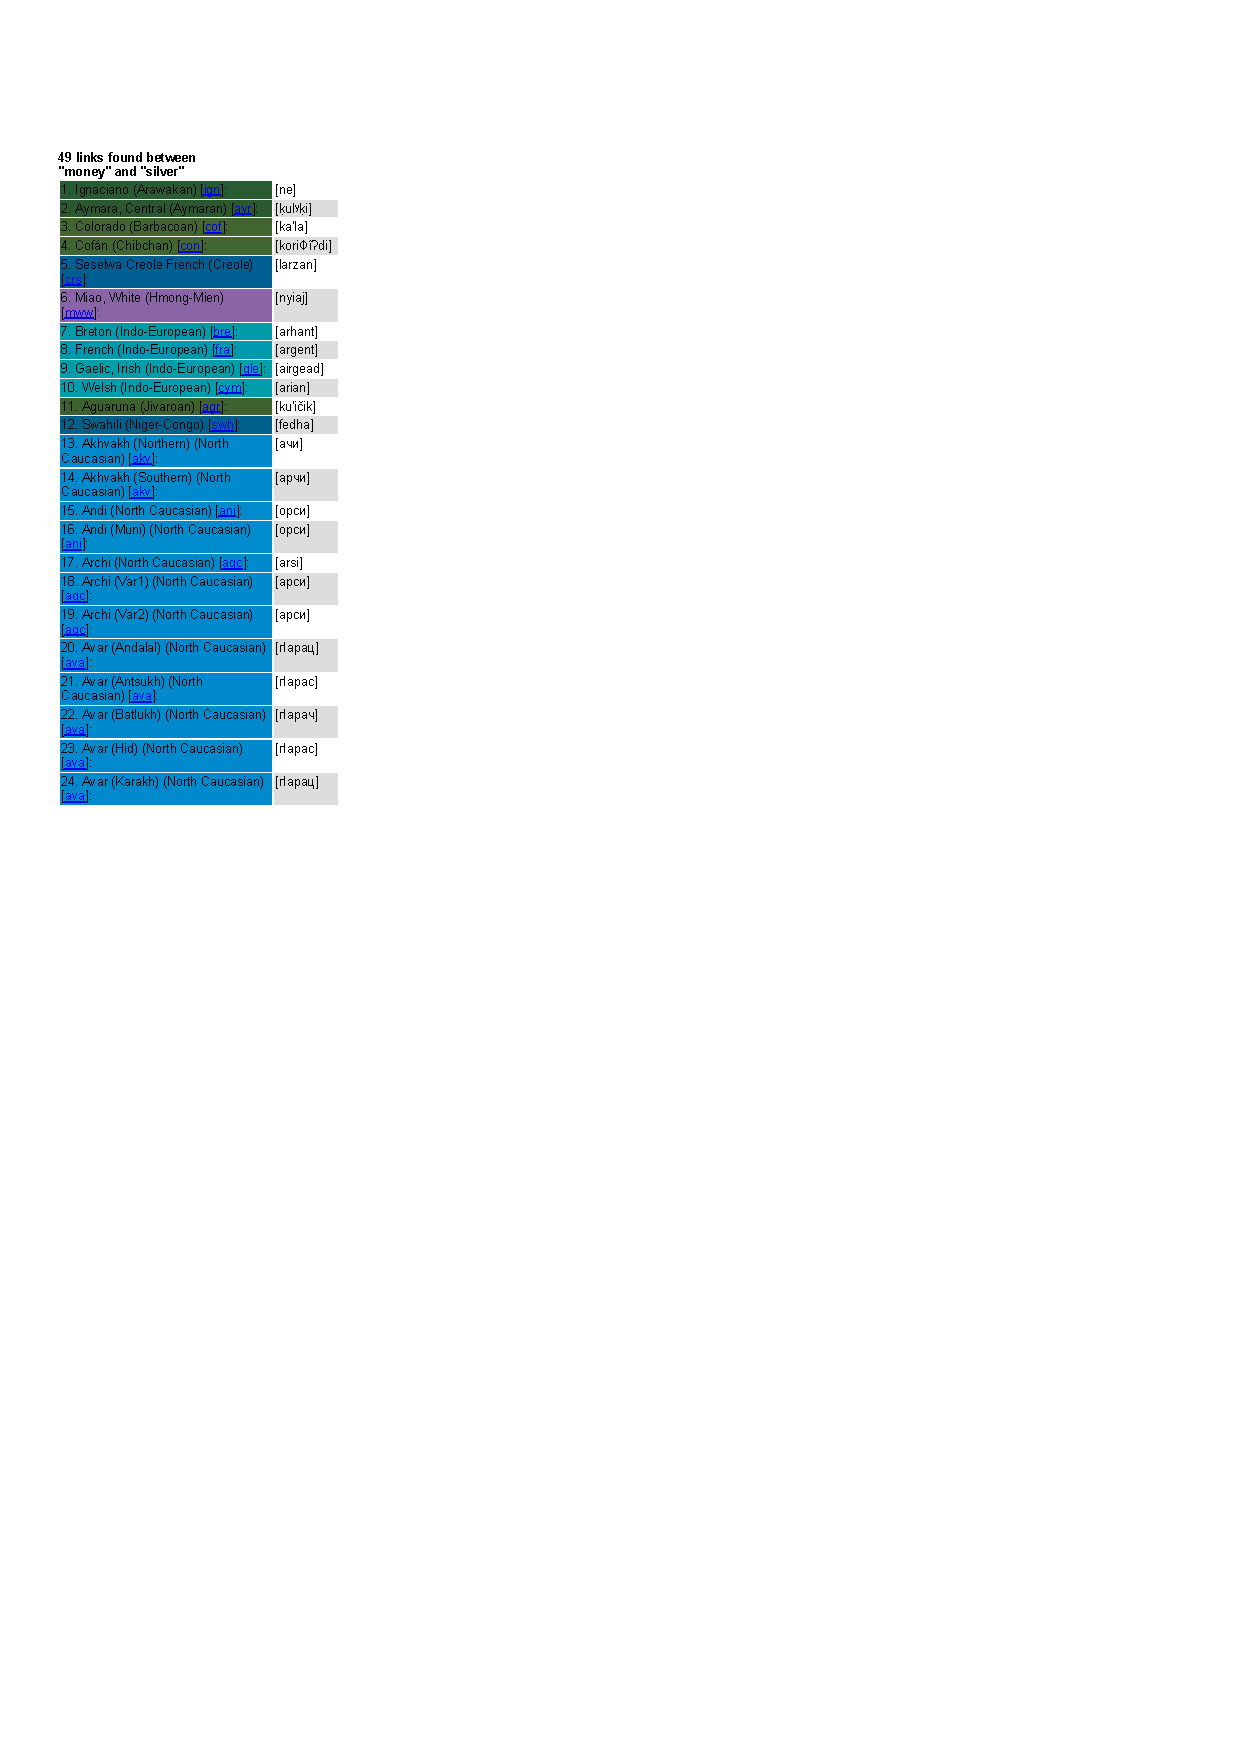
\includegraphics[width=0.238\textwidth]{img/moneysilverAreas1.pdf} &
\hspace{-0.2cm} \raisebox{2.8cm}{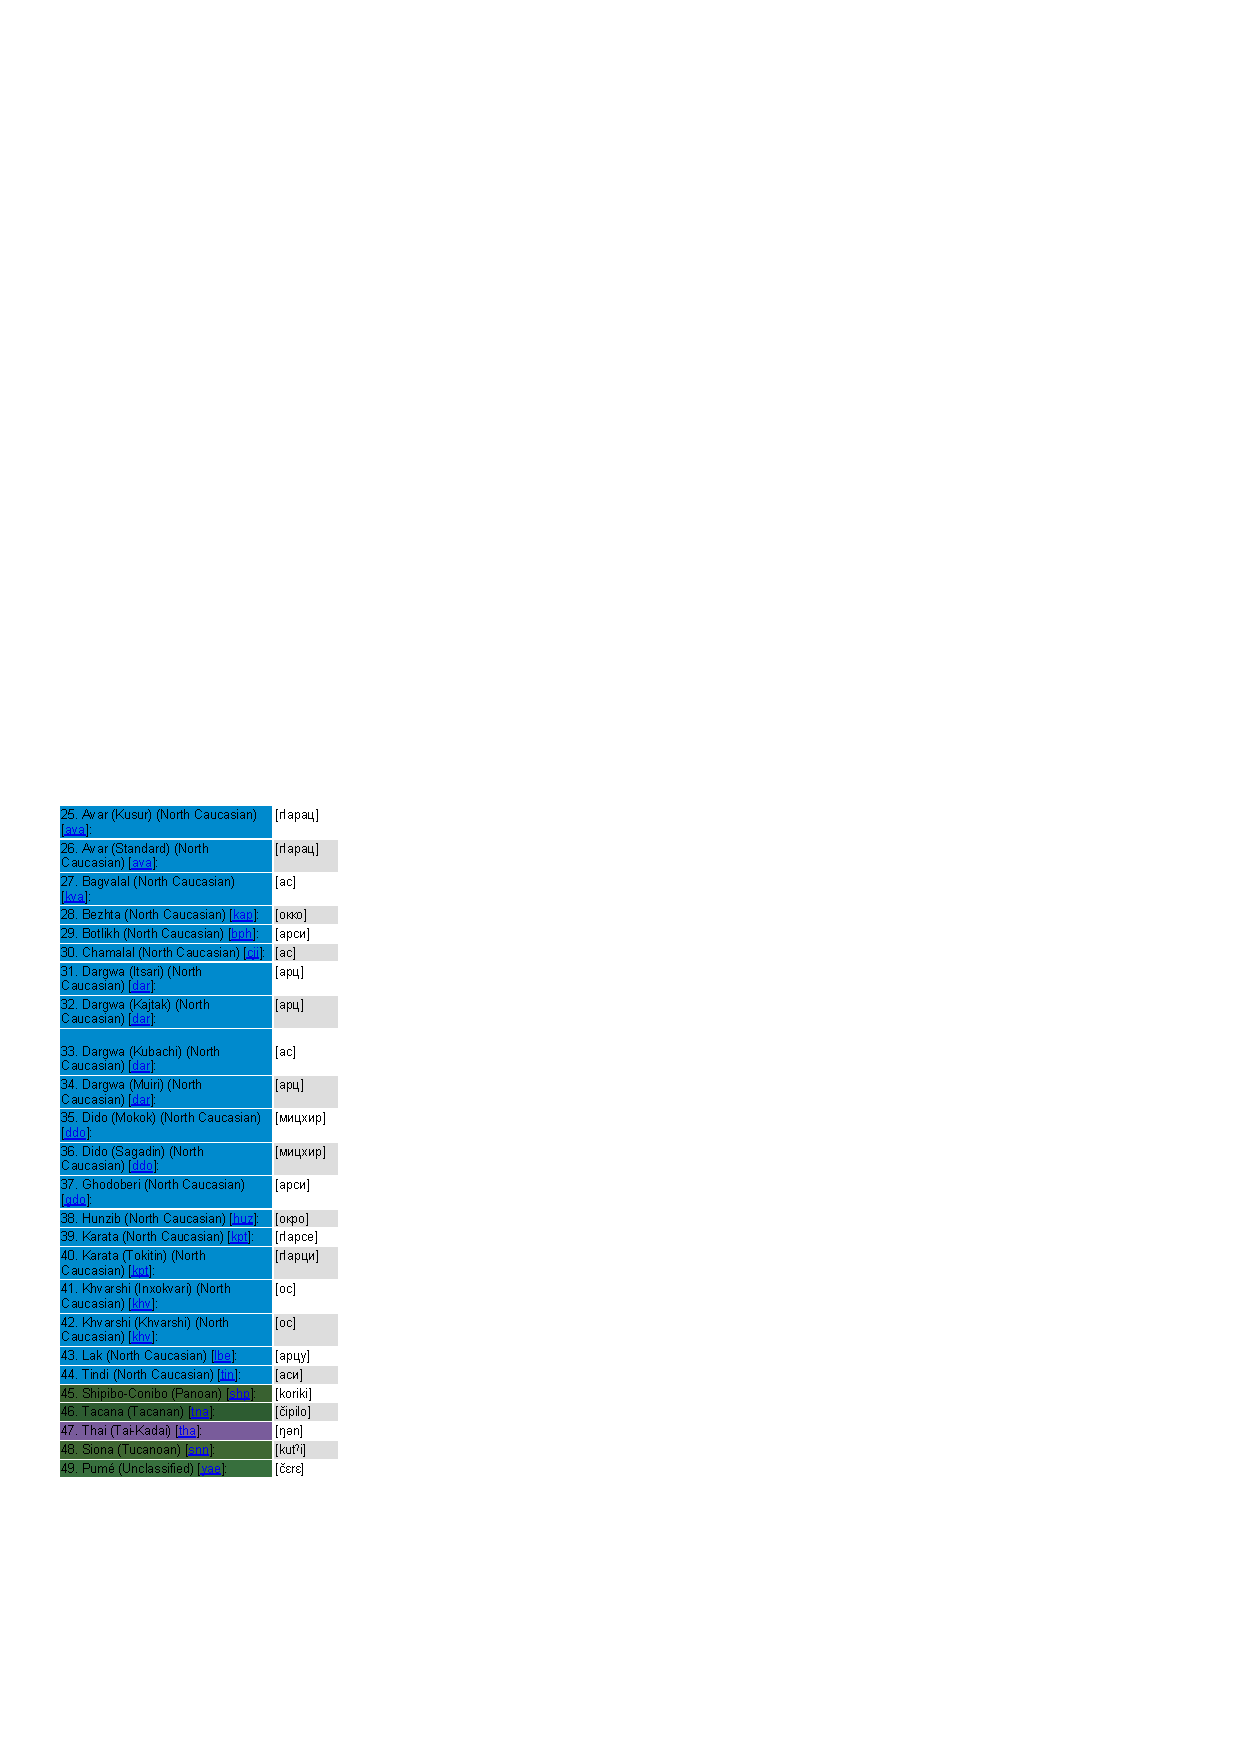
\includegraphics[width=0.238\textwidth]{img/moneysilverAreas2.pdf}}
\end{tabular}
\caption{Languages and words contributing to the connections of lexical associations for the concepts `money' and `silver'}
\label{MoneySilverAreas}
%\end{center}
\end{figure}

\begin{figure*}[htbp]
\begin{center}
    \href{\clics{browse.php?gloss=wheel&view=part}}{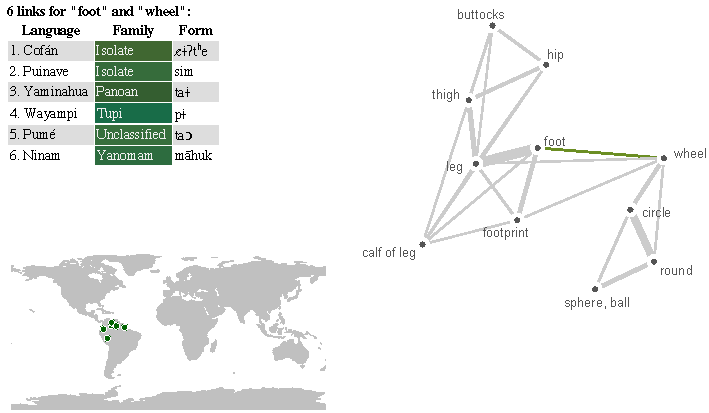
\includegraphics[width=\textwidth]{img/wheel-image.pdf}}
\caption{Force-directed graph with areal distribution for the concepts `wheel' and `foot.' In order
to browse the graph on the CLICS website, enter the following URL:
\url{\clics{browse.php?gloss=wheel&view=part}}.}
\label{WheelFootAreas}
\end{center}
\end{figure*}


Another example deals with the colexification of the concepts `wheel' and `foot.' In contrast to the case of `money' and `silver' above, these concepts at first glance may not immediately suggest a close association. Yet such cases do exist as the link in Figure \ref{WheelFootAreas} reveals. The connection links two bigger communities of nodes, including spherical objects on the one hand and parts of the lower body on the other. The list of languages for the connection `wheel' and `foot' in Figure \ref{WheelFootAreas} clearly shows that the association is restricted to languages of South America. 
This geographical restriction may reflect semantic borrowing among South American languages, but since the distribution within South America is rather erratic, independent innovation is also a possibility. At any rate, the color coding in the visualization immediately draws the researcher's attention to the potentially interesting geographical patterning.
%Even though the languages cover a range of different families, the areal distribution is clearly confined to a certain area. This might lead to the conclusion that the associations result from loan translations of the concept through language contact (the lexical entries show that they are most likely not cognates and that the association is thus due to loan words for both concepts). However, such a preliminary hypothesis has to be confirmed by looking at the actual data. 



